\documentclass[pdf]{beamer}
\usetheme{Madrid} % You can change this to other themes like Madrid, Copenhagen, etc.
\usecolortheme{default}
\usepackage{beamerthemesplit}
\usepackage{tabularx}
\usepackage{lscape}
\usepackage{graphicx}
\usepackage{tikz}\usetikzlibrary{arrows.meta,calc} %library tikz
% Packages for math and symbols
\usepackage{amsmath, amssymb}
\usepackage{graphicx} % For including images if needed
\usepackage[utf8]{inputenc}
\usepackage[dvipsnames]{xcolor}

% Title slide information
\title{Semi-stable lattices in higher rank}


\author{Tri Nguyen}


\begin{document}

% Title Slide
\begin{frame}
    \titlepage
\end{frame}

% Outline Slide
\begin{frame}{Outline}
    \tableofcontents
\end{frame}

\section{Introduction}
\begin{frame}{Historical motivation }
    Serre and Quillen used the notion of semistable vector
    bundle on an algebraic curve to study $\text{SL}_n(\mathcal{O})$ when $\mathcal{O}$ is a Dedekind domain finitely generated over a finite field. Stuhler
    then realized he can used the same method to adapt some work of Harder and Narasimhan on stable vector bundles to yields new facts
    about lattices in a Euclidean space.
\end{frame}

\begin{frame}{Definition of two-dimensional lattices}
    \begin{block}{Lattice}
        A lattice $L \subset \mathbb{R}^2$ is a set of the form
        \[L = \mathbb{Z}e_1\oplus\mathbb{Z}e_2\]
        where $e_1,e_2 \in \mathbb{R}^2$ are linearly independent over $\mathbb{R}$.
    \end{block}
\end{frame}
\begin{frame}{Example of a 2-dim lattice}
    \begin{figure}[h]
        \centering
        \resizebox{70mm}{70mm}{\begin{tikzpicture}
                \begin{scope}
                    \clip (0,0) rectangle (10cm,10cm); % Clips the picture...
                    \pgftransformcm{1}{0}{0.4}{1.5}{\pgfpoint{3cm}{3cm}} % Adjusted transformation matrix for less skew

                    \draw[style=help lines,dashed] (-14,-14) grid[step=1cm] (14,14); % Draws a grid in the new coordinates
                    \filldraw[fill=gray, draw=black] (0,0) rectangle (1,1); % Puts the shaded rectangle
                    \foreach \x in {-7,-6,...,7}{                           % Two indices running over each
                            \foreach \y in {-7,-6,...,7}{                       % node on the grid we have drawn 
                                    \node[draw,circle,inner sep=2pt,fill] at (\x,\y) {}; % Places a dot at those points
                                }
                        }
                    % Draw the vector from (0,0) to (1,0) in the transformed coordinate system
                    \draw[red, -Stealth, thick] (0,0) -- (1,0); % Vector from (0,0) to (1,0)
                    \draw[red, -Stealth, thick] (0,0) -- (0,1); % Vector from (0,0) to (0,1)

                \end{scope}
                % Place the circle at the lowest-left vertex (3,3) in the original coordinate system
                \fill[orange!50,semitransparent] (3,3) circle (.8cm); % Radius is 1.3cm to contain the shorter edge
            \end{tikzpicture}}
        \caption{Example of a lattice}
        \label{fig:example}
    \end{figure}
\end{frame}



\section{In 2 dimensions}
\begin{frame}{Classification of lattices}
    Do we know all the possible 2 dimensional "lattice shapes"?\vspace{3em}

    \pause
    \textbf{Answer:} Up to rescaling, rotation and change of basis, the answer is yes.
\end{frame}
\begin{frame}{Fundamental domain}
    Up to rotations and rescaling, we can reduce a lattice
    \[L = \mathbb{Z}e_1 \oplus \mathbb{Z}e_2\]
    to a lattice of the form
    \[L_z = \mathbb{Z}z\oplus\mathbb{Z}, \quad \Im(z)>0\]
    So the upper half-plane parametrizes the 2 dimensional lattices.
    \begin{block}{Classification of unit lattices}
        The map $z \mapsto L_z = \mathbb{Z}z\oplus\mathbb{Z}$ induces a bijection
        \[\text{SL}_2(\mathbb{Z}) \backslash\mathbb{H} \cong \left\lbrace \text{ lattices}\right\rbrace/\mathbb{C^\times}\]
    \end{block}

\end{frame}
\begin{frame}{Fundamental domain}
    So we reduce the study of the space of lattices by looking the action of $\text{SL}_2(\mathbb{Z})$ on the upper half plane. Geometrically, the fundamental domain is given by
    \[\mathfrak{D} = \left\lbrace z=x+iy \in \mathbb{H}: |z| \ge 1,-1/2 \le x \le 1/2 \right\rbrace \],
    \pause
    \[
        \begin{tikzpicture}[scale=2]
            \draw[densely dashed] (1,0) arc (0:60:1) (-1,0) arc (180:120:1);
            \draw[very thick, fill=gray!30] (.5,1.5) --node[right, pos=1]{$e^{2\pi i/6}=\rho$} (60:1) arc (60:120:1)
            --node[left, pos=.1]{$\rho^2=e^{2\pi i/3}$} (-.5,1.5);
            \draw[-latex] (-1.2,0) -- (1.2,0)node[below]{$\Re$};
            \draw[-latex] (0,-.2) -- (0,1.7)node[right]{$\Im$};
            \path(-1,0) --node[below, pos=0]{$-1$}node[below right, pos=.5]{0}node[below, pos=1]{1} (1,0)
            (0,1)node[below right]{$i$};
            \draw(-.5,.02)--(-.5,-.02)node[below]{$-\frac{1}{2}$}(.5,.02)--(.5,-.02)node[below]{$\frac{1}{2}$};
        \end{tikzpicture}\]
\end{frame}

\begin{frame}{Canonical plot}
    Grayson associated each lattice $L$  some kind of \textbf{Newton polygon}. \pause

    The process is as follows:
    \begin{enumerate}
        \item Put $(0,0)$ in the plot.
        \item For each primitive vector $v \in L$, he assigns the point $(1,\log(||v||))$ to the plot.
        \item Put the point $(2,\log(vol(L)))$ in the plot.
    \end{enumerate}
\end{frame}
\begin{frame}{Canonical plot}
    \begin{figure}[h]
        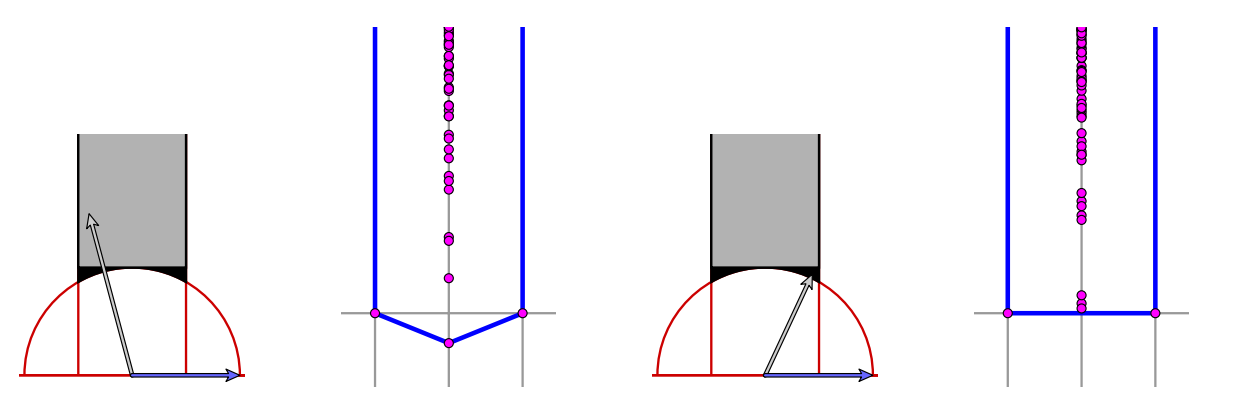
\includegraphics[width = \textwidth]{Canonical plot.png}
        \caption{\cite{casselman2004stability} - The figure on the left corresponds to $z = -2/5 +3i/2$ and on the right corresponds to $z = 7/16+15i/16$ }
    \end{figure}
\end{frame}
\begin{frame}{Canonical plot}
    Since the lattice is discrete, there is a shortest primitive vector - on the plot we have the lowest point on the vertical line $x=1$.\pause\vspace{3em}

    Grayson called the set of points plotted above as \textbf{canonical plot}. The convex hull of the collection
    of the plot points is called \textbf{profile}.
\end{frame}
\begin{frame}
    For any $z \in \mathbb{H} = \left\lbrace \text{Im}(z)>0 \right\rbrace$, we can assign to it a lattice of covolume $1$ as follows
    \[z \mapsto L_z = \mathbb{Z}\dfrac{e_1}{\sqrt{y}} + \mathbb{Z}\left(\dfrac{x}{\sqrt{y}}e_1+\sqrt{y}e_2 \right)\]
    The shortest vector is then $ e_1/\sqrt{y}$, with length $\dfrac{1}{\sqrt{y}}$. So for $y<1$, the lowest
    point is below the horizontal axis.
    \pause \vspace{2em}

    The element $z$ corresponds to a lattice $L_z$ such that its lowest point on the
    vertical line $x=1$ lies below the $x$-axis is called \textbf{semi-stable}, otherwise $z$ is called \textbf{unstable}.
\end{frame}
\begin{frame}{Semi-stable locus in fundamental domain}
    \begin{figure}{h}
        \begin{tikzpicture}[scale=2]
            \draw[densely dashed] (1,0) arc (0:60:1) (-1,0) arc (180:120:1);
            \draw[very thick, fill=gray!30] (.5,1.5) --node[right, pos=1]{$e^{2\pi i/6}=\rho$} (60:1) arc (60:120:1)
            --node[left, pos=.1]{$\rho^2=e^{2\pi i/3}$} (-.5,1.5);
            \draw[-latex] (-1.2,0) -- (1.2,0)node[below]{$\Re$};
            \draw[-latex] (0,-.2) -- (0,1.7)node[right]{$\Im$};
            \path(-1,0) --node[below, pos=0]{$-1$}node[below right, pos=.5]{0}node[below, pos=1]{1} (1,0)
            (0,1)node[below right]{$i$};
            \draw(-.5,.02)--(-.5,-.02)node[below]{$-\frac{1}{2}$}(.5,.02)--(.5,-.02)node[below]{$\frac{1}{2}$};
            \draw[red,thin,fill=blue] (-0.5,1) -- (0.5,1);
            \draw[very thick, fill = Turquoise](.5,1) -- (60:1) arc (60:120:1)
            -- (-.5,1);
        \end{tikzpicture}
        \caption{The blue part is the semistable locus in the fundamental domain}
    \end{figure}

\end{frame}
\begin{frame}
    Since the semi-stability is preserved under the action of $\text{SL}_2(\mathbb{Z})$, the semi-stable locus in the
    upper half plane $\mathbb{H}$ is as follows

\end{frame}
\begin{frame}
    \begin{figure}[h]
        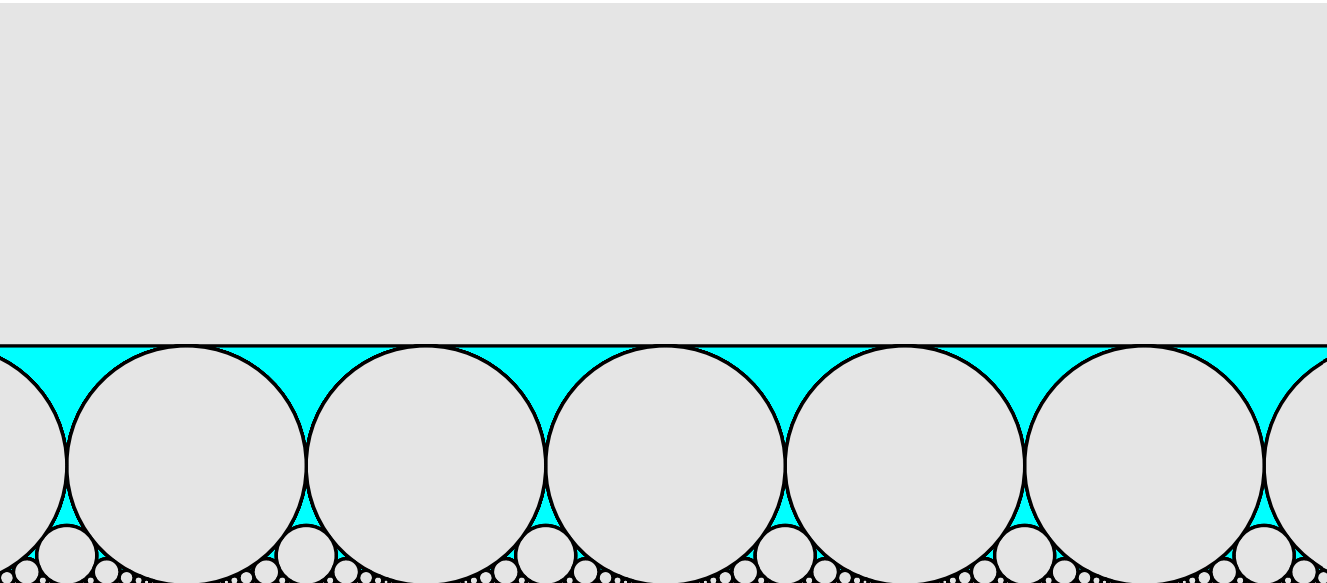
\includegraphics[width = \textwidth]{ss-locus.png}
        \caption{\cite{casselman2004stability} - Semi-stable locus over $\mathbb{H}$ - it is the complement of the union of the gray area }
    \end{figure}
\end{frame}
\section{In dimension at least 3}
\begin{frame}{In higher dimensions}
    We work with the lattices of the form $g\mathbb{Z}^n$ for $g \in \text{GL}_n(\mathbb{R})$ or
    $g \in \text{SL}_n(\mathbb{R})$. The latter yields lattices with unit volumes. Even if we want to work with unit lattices,
    we still need to consider the sublattices of arbitrary volumes.
    \pause
    \begin{block}{Sublattice}
        A discrete subgroup $M$ of the lattice $L$ is called \textbf{sublatice} if it satisfies one of the
        the following equivalent conditions:
        \begin{enumerate}
            \item $L/M$ is torsion-free.
            \item $M$ is a direct summand in $L$.
            \item Every basis of $M$ can be extended to a basis in $L$.
            \item The quotient $L/M$ is a free $\mathbb{Z}-$module.
        \end{enumerate}
    \end{block}
\end{frame}
\begin{frame}{Volume of lattice}
    The volume of $L = g\mathbb{Z}^n$ is just $\det(g)$. Assume that $M$ is a sublattice of $L$ of rank $k \le n$
    with a basis
    \[\left\lbrace v_1, v_2,\ldots, v_k\right\rbrace\]
    Let $e_1,e_2,\ldots,e_n$ be the standard basis in $L \otimes \mathbb{R} \cong \mathbb{R}^n$. We can form a matrix of size $k \times n$
    \[A = \begin{bmatrix}
            \left\langle v_i ,e_j\right\rangle
        \end{bmatrix}\]
    The volume of $M$ is defined to be the sum of the squares of the determinants of the $k \times k$ minor matrices in the matrix $A$.
    % Add an example on the board here. 
\end{frame}
\begin{frame}{Canonical plot in higher dimension}
    Grayson assigns to the lattice $L$ a canonical plot as follows:
    \begin{enumerate}
        \item Put the point $(0,0)$ in the plot.
        \item For each sublattice $M \subset L$, assign a point with coordinates ${l}(M) = (\text{rank}(M), \log(\text{vol}(M)))$ to the plot.
        \item Put the point $(n, \log(\text{vol}(L)))$ in the lattice.
    \end{enumerate} \pause

    As before, we call the convex hull of this plot its \textbf{profile}.
\end{frame}
\begin{frame}
    We have the following proposition:
    \begin{block}{Lemma - Grayson}
        Fix a lattice $L$ of rank $n$ and a positive number $c$. For each $k \leq n$, there are only finitely many sublattices $M \subset L$ such that
        $\text{vol}(M) < c$.
    \end{block} \pause

    This guarantees that on each vertical line $x = k$, there exists a lowest point corresponding to the sublattice of smallest volume of each rank $k$.
    In particular, the bottom of the profile is bounded below. Hence, the following definition makes sense: \pause
    \begin{block}{Semi-stable lattice}
        A lattice $L$ is called \textbf{semi-stable} if the bottom of the profile is just a line.
    \end{block}
\end{frame}
\begin{frame}{Example of a higher rank profile}
    \centering
    \begin{figure}
        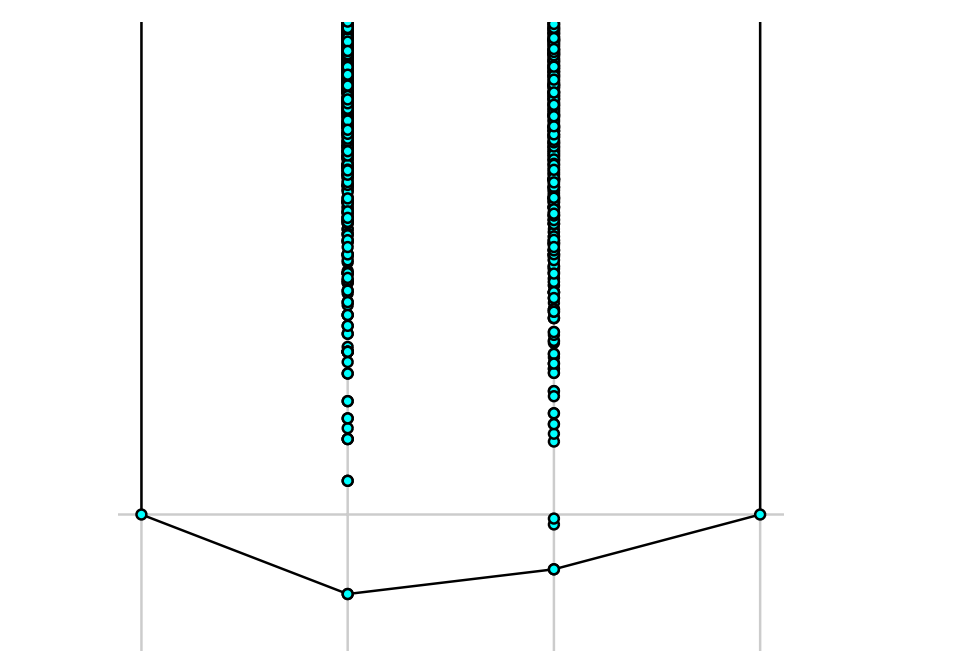
\includegraphics[width = 0.7\textwidth]{Canonical plot 3 dim.png}
        \caption{An unstable lattice}
    \end{figure}
\end{frame}
\begin{frame}{Iwasawa decomposition}
    We recall the Iwasawa decomposition for $G = \text{GL}_n$:
    \[G = K \times A \times N\]
    where:
    \begin{enumerate}
        \item $K$ is the orthogonal subgroup.
        \item $A$ is the group of diagonal matrices with positive entries along the diagonal.
        \item $N$ is the unipotent subgroup.
    \end{enumerate}
\end{frame}
%give example for GL_2
\begin{frame}{Parabolic subgroups}
    For $G =\text{GL}_n$ we have an explicit description of standard parabolic subgroups
    \pause\begin{block}{Standard Parabolic subgroups of $\text{GL}_n$}
        For each partition
        $$n = n_1+n_2+\ldots+n_k$$
        We denote $P_{n_1,n_2,\ldots,n_k}$ the standard parabolic subgroup of type $(n_1,\ldots, n_k)$ to be the subgroup of
        matrices of the form
        \[P_{n_1,\ldots, n_k} = \left\lbrace \begin{bmatrix}
                \mathfrak{m}_1 & \ast           & \ldots & \ast           \\
                0              & \mathfrak{m}_2 & \ldots & \ast           \\
                \vdots         & \vdots         & \ddots & \vdots         \\
                0              & 0              & \ldots & \mathfrak{m}_k
            \end{bmatrix} \right\rbrace\]
        where $\mathfrak{m_i}$ is invertible of size $n_i \times n_i$.
    \end{block}
\end{frame}
\begin{frame}{Degree of instability}
    Now we are ready to define the degree of instability
    \begin{block}{Degree of instability, \cite{chaudouard2016variante}}
        For each $x \in G$, we define its degree of instability to be
        \[\deg_{\text{inst}}(x):= \min_{P \in \text{ParSt}, \gamma \in G/P}\left\langle\rho_P, H_B(x\gamma) \right\rangle \]
    \end{block}\pause
    We define the notion of $\rho$-semistable as follows
    \begin{block}{$\rho$-semistable}
        A point $x \in G$ is called \textbf{semi-stable} iff $\deg_{\text{inst}}(x) \ge 0$.
    \end{block}
\end{frame}
\begin{frame}{Equivalent between two notions of semi-stable}

    We have
    \[\left\langle \rho_{Q_i}, H_B(x\gamma)   \right\rangle = a_1a_2\ldots a_i\]\pause
    where
    \[x = k_xa_xn_x \in K \times A \times N,\]
    in which
    \[a_x = \begin{bmatrix}
            a_1    & 0      & \ldots & 0      \\
            0      & a_1    & \ldots & 0      \\
            \vdots & \vdots & \ddots & \vdots \\
            0      & 0      & \ldots & a_n
        \end{bmatrix}\]
\end{frame}
\begin{frame}{Equivalent between two notions of semi-stable lattices}
    We have the following Lemma
    \begin{block}{Lemma 2.2.1, \cite{chaudouard2016variante}}
        The following are equivalent:
        \begin{enumerate}
            \item \(\deg_{\text{inst}}(x) \geq 0\);
            \item For every parabolic subgroup \( P \subset G \), every \( \delta \in G(\mathbb{Q})/P(\mathbb{Q})\), and every \( \varpi \in \hat{\Delta}_P^G \), we have:
                  \[
                      \langle \varpi, H_B(x\delta ) \rangle \geq 0;
                  \]
            \item For every maximal parabolic subgroup \( P \subset G \), every \( \delta \in  G(\mathbb{Q})/P(\mathbb{Q})\) , and every \( \varpi \in \hat{\Delta}_P^G \), we have:
                  \[
                      \langle \varpi, H_B(x\delta ) \rangle \geq 0.
                  \]
        \end{enumerate}
    \end{block}
\end{frame}


\begin{frame}
    This suggests that there should be a connection between the maximal parabolic subgroups of $G$
    and sublattices of $L$. Indeed we have
    \[ \text{GL}_n(\mathbb{Z})/(Q_i(\mathbb{Q}) \cap \text{GL}_n(\mathbb{Z})) \longleftrightarrow \left\lbrace \text{ sublattices of rank $i$ of $\mathbb{Z}^n$}\right\rbrace\]

    So we have the main theorem
    \begin{block}{Main theorem}
        Let $x \in X_n = K \backslash \text{GL}_n(\mathbb{R})$ - the space of lattices . Then $x$ is semi-stable if one of the following equaivalent
        conditions holds
        \begin{enumerate}
            \item The bottom of the profile of the lattice corresponding to $x$ is a straight line that connects the origin and $(n,\log(\text{vol}(L)))$.
            \item The degree of instability of $x$ is nonnegative, namely, $\deg_{\text{inst}}(x) \ge 0$.
        \end{enumerate}
    \end{block}

\end{frame}
\begin{frame}{References}
    \bibliographystyle{plain} % We choose the "plain" reference style
    \bibliography{refs} % Entries are in the refs.bib file

\end{frame}

\begin{frame}
    \begin{center}
        \textit{THANK YOU FOR YOUR ATTENTION.}
    \end{center}
\end{frame}

\end{document}
\begin{frame}
    Due to \cite{borek2005successive} , it is heuristic that the semi-stable lattices are the lattices in which the successive minima are closed.
\end{frame}